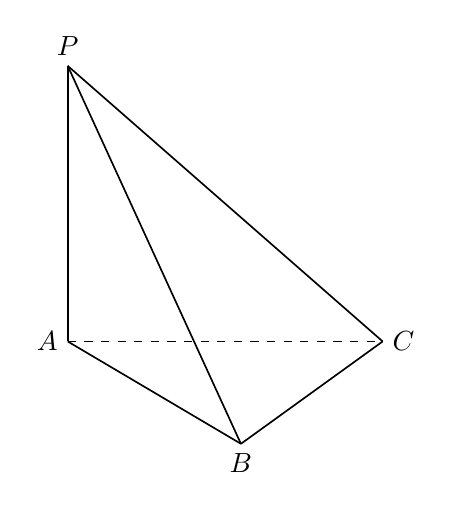
\begin{tikzpicture}[line width=0.6pt]
\coordinate (P) at (0,4);
\coordinate (A) at (0,0.5);
\coordinate (C) at (4,0.5);
\coordinate (B) at (2.2,-0.8);
% visible edges solid
\draw[solid] (P) -- (A);
\draw[solid] (P) -- (B);
\draw[solid] (P) -- (C);
\draw[solid] (A) -- (B);
\draw[solid] (B) -- (C);
% hidden edge AC dashed
\draw[dashed] (A) -- (C);
% labels
\node[above] at (P) {$P$};
\node[left] at (A) {$A$};
\node[right] at (C) {$C$};
\node[below] at (B) {$B$};
\end{tikzpicture}
